
\section{Antenna} \label{sAntenna}

The DC voltage supplied to the antenna is selectable as either 3.3 or 5 V with the jumper J1. 
The default is 5 V. Short circuit protection is 
provided via the $1 \Omega$ fusible resistor R25.

The NV08C-CSM has two antenna inputs ANT-A (active) and ANT-P (passive).
When the antenna is connected to ANT-P (default setting) the external DC power supply is used.
If the antenna is connected to ANT-A, the NV08-CSM board supplies 3.3 V DC and
short circuit protection is provided by the board.


\begin{figure}

	\centering
	
	\begin{subfigure}[t]{6cm}
		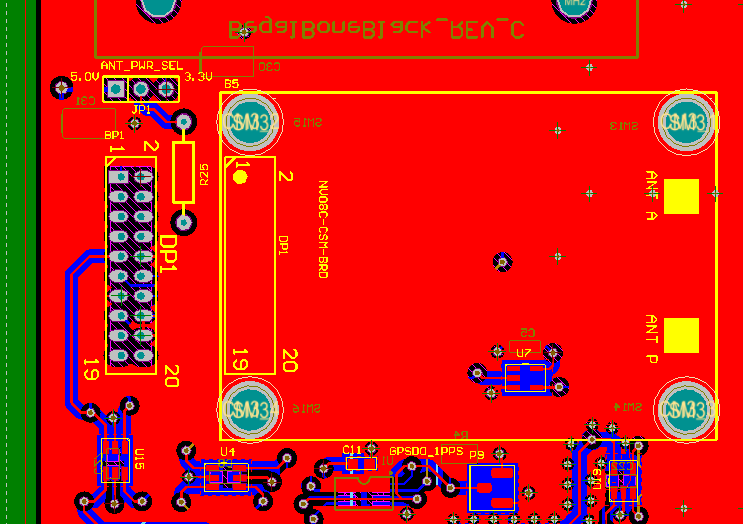
\includegraphics[width=6cm]{figures/antennavselpcb.png}
		\caption{Location of JP1 }
	\end{subfigure}
	
	\quad

	\begin{subfigure}[t]{6cm}
		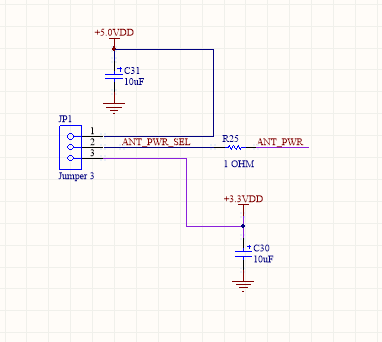
\includegraphics[width=6cm]{figures/antennavselcircuit.png}
		\caption{JP1 voltages}
	\end{subfigure}
	
	\caption{Selection of antenna voltage using JP1}
	
\end{figure}
